\documentclass[./main.tex]{subfiles}

\begin{document}
\section{Discussion}\label{sec:discussion}
In the following we will be discussing our procedure as well as our results. We will start off in Section \ref{subsec:summary}, where we will be giving a brief summary of our obtained results from Section \ref{experiement}, \ref{sec:XAI} and \ref{sec:improving}. We will then in Section \ref{subsec:comparisons} compare our results with the results of Newell \textit{et al.} \cite{Newell} and Olsen \cite{Camilla}, as well as discuss the differences in the results. In Section \ref{subsec:XAI_disc} we will be discussing our interpretation of the Stacked hourglass, including our approach as well as the results. In Section \ref{subsec:why_improvement} we will argue and discuss why the autoencoder improved our initial model. Lasty, we will in Section \ref{subsec:Future_work} comment on potential future work in relation to this project.

\subsection{Summary of the Obtained Results}\label{subsec:summary}
In Section \ref{experiement}, we succefully implemented and trained a Stacked hourglass, consisting of a single hourglass. We did this by following the configuration details described by Newell \textit{et al.} \cite{Newell} and Olsen \cite{Camilla}. The developed model has a validation PCK accuracy of $0.433$ and a test PCK accuracy of $0.441$. 
\\
\\
In Section \ref{sec:XAI} we gained an understanding of how the devleoped model works by exploring the different components of the model. We could verify, that the skip-connections of the model were used for recreating details that are lost during the encoder-phase of the model, as claimed by Newell \textit{et al.} \cite{Newell} and Olsen \cite{Camilla}. We then used PCA to gain an understanding of the structure of the latent space of the model. By doing so we came to the conclusion, that the first principal component of the latent space is used for deciding if a given person is sitting down or standing up,, as well as possibly discovering some redundancy in the model, as principal componet $50$ and above seemed to act as noise. Lastly, we clustered the latent space to gain an understanding of how the model works. By doing so we learned, that the model knows the difference between fully-annotated people and not-fully annotated people, as well as knows the difference between stationary people and moving people. Here we also identified some possible reasons for inaccuracies of the model, as these groupings are not always correct.
\\
\\
In Section \ref{sec:improving}, we used our knowledge of the model to improve the performance of the model. This was done by developing and training an autoencoder, which was placed in the model. We decided to make use of an autoencoder, as we knew from the previous section, that the latent space of the Stacked hourglass contained a lot of noise, as well as some missclassifications, which the autoencoder possibly could help on. By doing so, both the validation and test PCK accuracy increased to $0.467$ and $0.473$, respectively.

\subsection{Comparison of Models}\label{subsec:comparisons}
\begin{table}[htbp]
    \begin{tabular}{l|c|c}
        Description & \# stacks & Testing accuracy \\
        \hline
        Olsen - $2A$ & $2$ & $0.72$ \\
        \hline
        Olsen - $2B$ & $2$ & $0.81$ \\
        \hline
        Olsen - $2M$ & $2$ & $0.83$ \\
        \hline
        \hline
        Our SHG & $1$ & $0.469$ \\
        \hline
        \textbf{Our modified SHG} & $\bm{1}$ & $\bm{0.576}$ \\
        \hline
    \end{tabular}
    \caption{Comparison of our developled models with Olsens developed model \cite{Camilla}. The testing accuracy is only based on fully-visible joints (that is, where $v = 2$)}.
    \label{fig:Olsen_comparison}
\end{table}
\noindent To further understand the performance of our developed models, we have in Table \ref{fig:Olsen_comparison} compared our models with the models developed by Olsen \cite{Camilla}, which consisted of $2$ stacks.
\\
\\
By looking at Table \ref{fig:Olsen_comparison} we see, that the performances of the models developed by Olsen \cite{Camilla} exceeds the performances of our developed models. However, we also see, that all of Olsen's \cite{Camilla} models use more stacks, than our models, which could explain the better performance. This is also argued by Newell \textit{et al.}, as they describe how stacking multiple hourglasses, increases the performance of the model \cite{Newell}.
\\
\\
Another reasoning behind the loss of performance compared with the models developed by Olsen \cite{Camilla} is, that Olsen's models were only trained on fully-visible joints \cite{Camilla}, whereas our models were trained on both fully-visible joints and on non-visible joints. This could make Olsen's models \cite{Camilla} perform better on fully-visible joints, as this probably makes the model more focused on learning fully-visible joints during training. We would thus argue, that if we were to retrain our models on only fully-visible joints, the gap between the performance of our models and Olsen's models \cite{Camilla} would become smaller, and even very small in the case of the modified Stacked hourglass. This is however not possible to predict and thus only purely speculation, however, our thought experiment does support this claim.
\\
\\
Olsen's models and data are more similar to ours, than the ones used by Newell \textit{et al.} \cite{Newell}, making the comparison more accurate. However, we can still compare our results with the ones obtained by Newell \textit{et al.} \cite{Newell} to get a further performance evaluation of our models.
\\
\\
Like in our case, Newelll \textit{et al.} do also develop a model consisting of only a single hourglass. However, Newell \textit{et al.} does not report the testing accuracy of this model. Instead, they report the evolution of the validation accuracy during training, for joints that are not associated with the head and torso. The validation accuracy seems to top at around $0.65$ \cite{Newell}. If we test our models on the joints from our testing data, that are not associated with the head or torso, we get a PCK accuracy of $0.32$ and $0.38$ for the Stacked hourglass and the modified Stacked hourglass, respectively.
\\
\\
There are a number of reasons that could explain the poor performance of our models compared with the models developed by Newell \textit{et al.} \cite{Newell}. 
\begin{enumerate}
    \item We use a different dataset than Newell \textit{et al.} \cite{Newell}: Newell \textit{et al.} uses the FLIC \cite{FLIC} and MPII Human Pose \cite{MPII} datasets, whereas we use the 2017 Microsoft COCO dataset \cite{COCO_article}. These datasets could potentially be different from the dataset that we use, making it an unfair comparison to compare our results with Newell \textit{et al.}'s results \cite{Newell}. For instance, the FLIC \cite{FLIC} and MPII Human Pose \cite{MPII} could contain less occlusion than the Microsoft COCO dataset \cite{COCO_article}, which would decrease the performance of our model, as argued by Newell \textit{et al.} \cite{Newell}.
    \item Our preprocessing of not-visible joints was different than the preprocessing done by Newell \textit{et al.} \cite{Newell}: when we preprocessed the data, we made use of a Guassian filter to represent uncertainty in the annotation. For not-visible joints we used a standard deviation of $0.5$, whereas we for visible joints used a standard deviation of $1$. Newell \textit{et al.} describes, how they for all joints used a standard deviation of $1$ \cite{Newell}. We decided to use a standard deviation of $0.5$ for not-visible joints, as the uncertainty of the annotation of these joints is greater, than for visible joints. This could however also possibly have confused the model, as it thus implicitly also learns to predict whether a given joint is visible or not, making the complexity of the model greater, possibly decreasing the performance of the model.
    \item We use a different PCK accuracy metric: Newell \textit{et al.} state, that they use different PCK accuracy metrics - that is PCK accuracy metrics, where the normalization constant is different - at different times \cite{Newell}, however, they do not state which PCK accuracy metric they used for validation during training. We chose a normalization constant equal to one tenth of the heatmap size, however, if Newell \textit{et al.} \cite{Newell} used a greater normalization constant, the predictions would have a bigger probability of being accepted as correct, making the accuracy of the developed model seem greater than it actually is. Likewise, Newell \textit{et al.} \cite{Newell} do not state the threshold radius they use. If they were to use a threshold radius greater than the one we use, their estimations have a greater probability of being counted as correct, than our estimations.
    \item Newell \textit{et al.} describes that they use batch normalizations to prevent the model from overfitting, however, they do not describe where they used these batch normalizations \cite{Newell}. If we were to place our batch normalizations at places different than where Newell \textit{et al.} \cite{Newell} place theirs, we could make our model overfit much quicker than what Newell \textit{et al.} \cite{Newell} experiences, resulting in worse performance. This, however, is much less likely, as we decided to follow Olsen \cite{Camilla} for the placement of batch normalization and they achieved great results, hinting towards their, and thus also our, placements of the batch normalizations being correct.
    \item We use different configurations: Newell \textit{et al.} \cite{Newell} does not state the decay rate $\rho$ for RMSProp. We decided to use a decay rate of $0.99$, as this is the default value in PyTorch, resulting in a slow decay of the accumulated squared gradient $\bm{r}$. If Newell \textit{et al.} \cite{Newell} use a different value for the decay rate, $\bm{r}$ would most likely decay differently, potentially resulting in different results. Likewise, Newell \textit{et al.} \cite{Newell} does not state how they initialize the parameters of their model, hence why, the differences in performance could be explained by a potentiel difference in how they initialize the parameters in their model and in how we initialize the parameters in our model. This is however, not likely to have a big impact on the results, as Olsen \cite{Camilla} performed the same method for initializing the parameters of their model as we did and received great results, making us believe, that our method for initialization should not be a problem.
\end{enumerate}
Overall, the comparison between our developed model and the model developed by Newell \textit{et al.} \cite{Newell} is difficult, as they have a lot of differences. The comparison between our model and Olsen's model \cite{Camilla} is thus more accurate, however, still inaccurate, as Olsen's models use $2$ stacks instead of just $1$ as in our case \cite{Camilla}.

\subsection{How Good was the Interpretation of the Stacked Hourglass?}\label{subsec:XAI_disc}
In Section \ref{sec:XAI} we interpretated the Stacked hourglass developed in Section \ref{experiement}. In the following we will be discussing our approach, as well as the obtained results.

\subsubsection{Verification of the Skip-Connections}
In Section \ref{subsec:verifying_skip_cons} we verified the effects of the skip-connections of the Stacked hourglass. This was done by disabling the skip-connections of the already trained Stacked hourglass and comparing the corresponding results with results of the the Stacked hourglass with the skip-connections enabled. This approach however, is not optimal, as we will be having some biased results, due to the fact, that the network was trained with the skip-connections enabled. Our approach does give a brief view into the effects of the skip-connections, however, to get an understanding of the full effects of the skip-connections, we should have trained a Stacked hourglass with the skip-connections disabled, whose results should have been compared with the Stacked hourglass with the skip-connections enabled.

\subsubsection{Dimensionality Analysis of the Latent Space}
\begin{figure}[htbp]
    \centering
    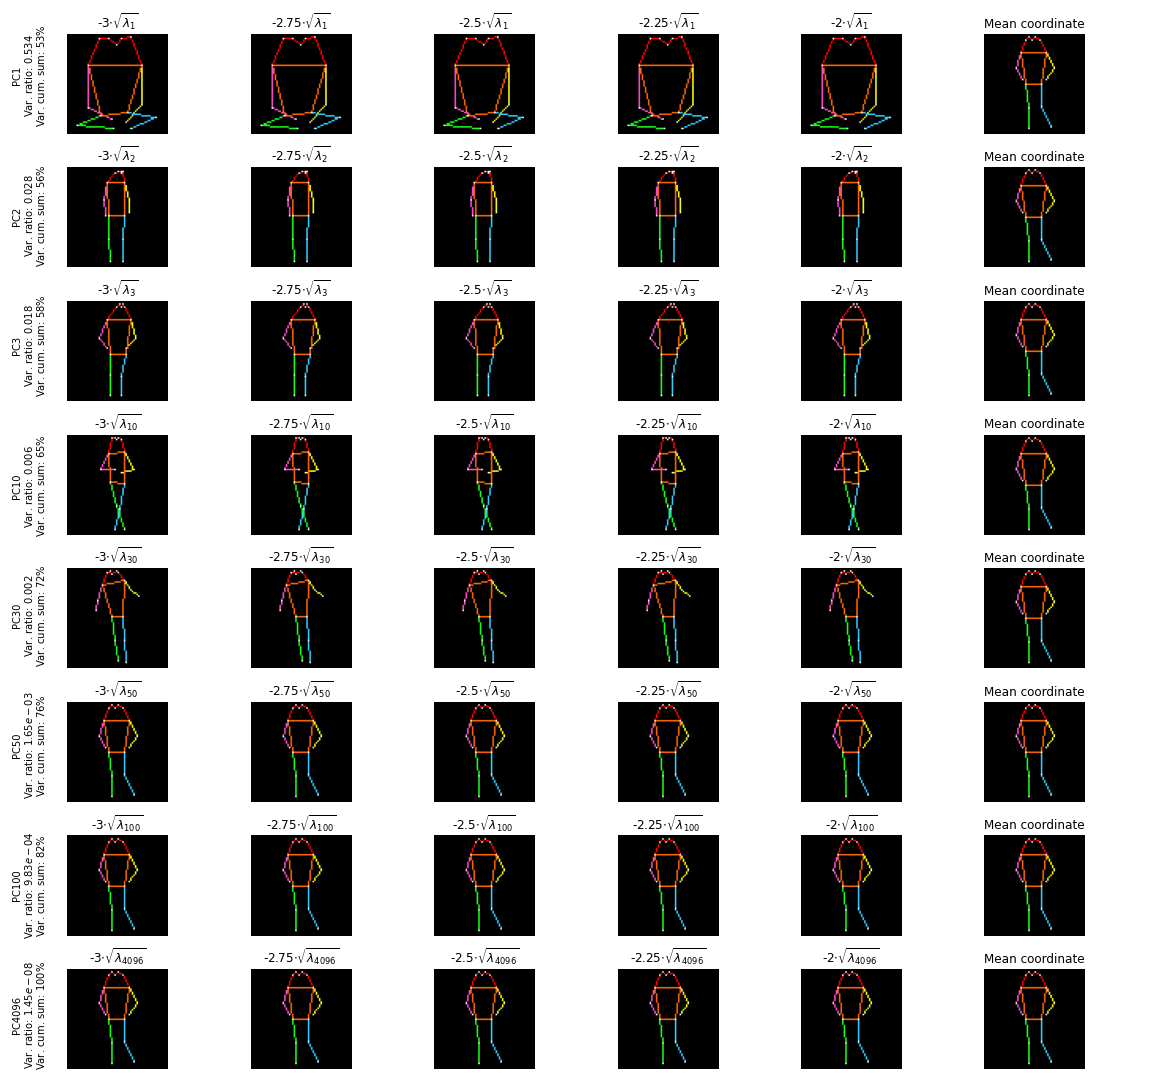
\includegraphics[width = \textwidth]{entities/shape_analysis_2.png}
    \caption{Nearest observation to the end of "walking" along various principal component with small step sizes.}
    \label{fig:shape_analysis_2}
\end{figure}
\noindent In Section \ref{subsec:shape_analysis} we looked at the effects of various principal components of the latent space of the developed Stacked hourglass. We did this by "walking" along a given principal component with a step size of the form $c \cdot \sqrt{\lambda}$, where $c$ is a constant and $\lambda$ is the explained variance of the corresponding principal component. By looking at the results of walking in Figure \ref{fig:shape_analysis} we see, that all of the results of walking in negative direction with a step size of $c = 3$ yields the same results as walking in negative direction with a step size of $c = 2$. This hints towards, that the increase of $c$ is to great and we thus are missing some important information, which potentially could disproof our claim that principal component $50$ and forward are just noise. However, we have in Figure \ref{fig:shape_analysis_2} visualized the effects of "walking" with a smaller increase of $c$ to explore the data in between $c = 2$ and $c = 3$. By doing so we can clearly see, that we did not miss any important information when we performed the dimensionality analysis in Section \ref{subsec:shape_analysis}, as the extra steps between $c = 2$ and $c = 3$ do not add extra information.

\subsubsection{Clustering the Latent Space}
In Section \ref{subsec:clustering} we used clustering on the latent space of the developed Stacked hourglass to get an understanding of how the model works. Due to memory constrains we only included $10.000$ training samples of the total $124.040$ training samples.  One could argue, that this would result in unreliable results, as only a minor subset of the dataset is used and clustering on the whole dataset could result in different results, such as the optimal amount of clusters would be more than $2$ according to the Silhouette score. Due to our memory constraint, this is not easily verifiable, however, if we take a look at \textit{Cluster 0} in Figure \ref{fig:clusters_all_skeletons}, we can see, that the cluster can be somewhat split into two parts; one minor part in the top left and one greater part in the center/bottom left, hinting towards the true amount of clusters is actually $3$ instead of $2$. This does not verfy the argument of the unrelaible results, however, it does defiently support it. Whether the increase of observations would have an effect on the clustering is difficult to say, however, it is defiently possible.

\subsection{Why did the Autoencoder Improve the Stacked hourglass?}\label{subsec:why_improvement}
In Section \ref{subsec:improv_motivation} we argued the following two reasons for why using the autoencoder could improve the performance of the model: $(1)$ inconsistency of the placement of the training observations, and $(2)$ having principal components that acts as noise. In the following we will be analysing and discussing our results of using the autoencoder, leading to if these two reasons actually had an effect on the performance of the model.
\subsubsection{Clustering the Latent Space}
\begin{figure}[htbp]
    \centering
    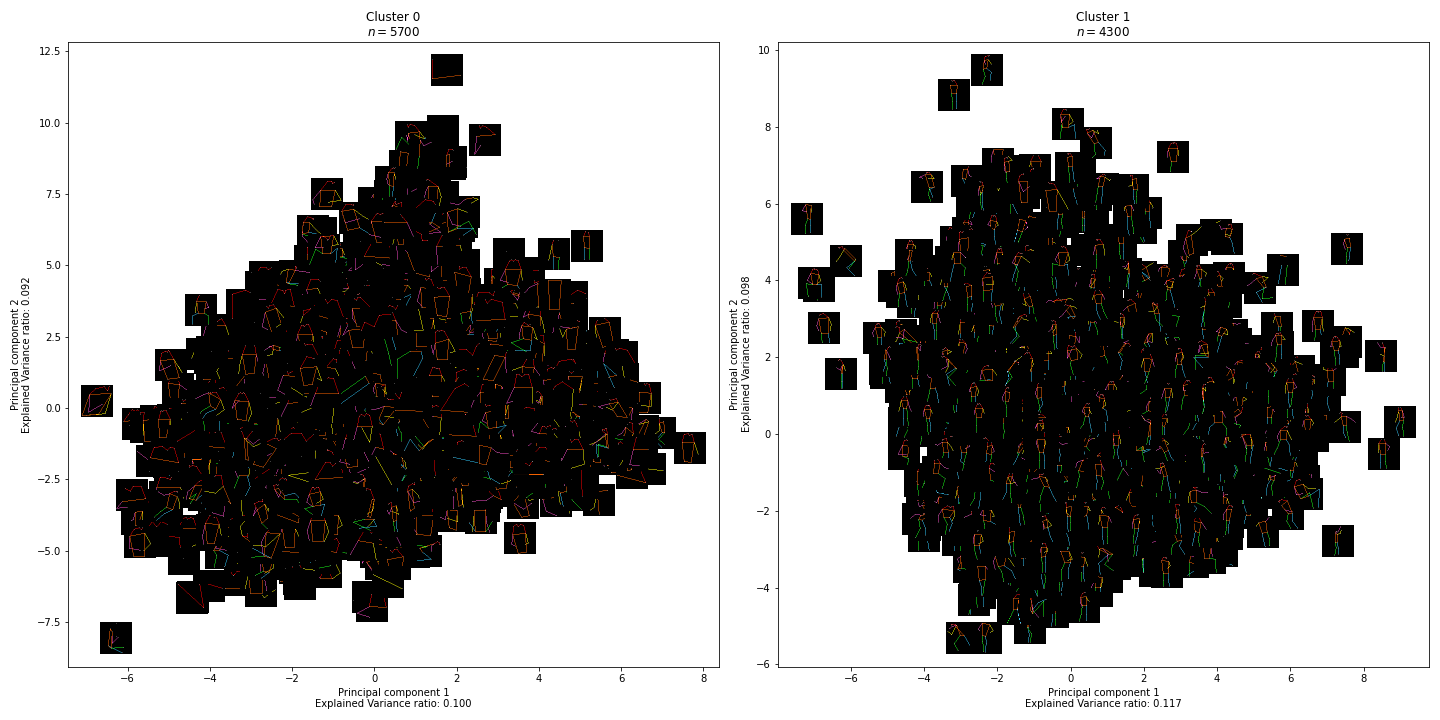
\includegraphics[width = \textwidth]{./entities/SHG_AE_clusters.png}
    \caption{Results of performing $K$-Means clustering on $10.000$ random samples of the latent space of the autoencoder}
    \label{fig:SHG_AE_clusters}
\end{figure}
\noindent In Figure \ref{fig:SHG_AE_clusters}, we have visualized the results of performing $K$-Means on the latent space of the autoencoder with $K = 2$. Due to memory limitations only $10.000$ training samples were used. 
\\
\\
In Figure \ref{fig:clusters_all_skeletons} we visualized equivalent results of performing the same procedure on the latent space of the Stacked hourglass. In correlation to Figure \ref{fig:clusters_all_skeletons} we argued, that the two clusters contained some missclassifications, which could explain the poor performance of the model. More specifically, \textit{Cluster 1}, the cluster containing samples with a lot of keypoints missing, contained a lot of samples that should ideally have been in \textit{Cluster 0}.
\\
\\
If we compare Figure \ref{fig:SHG_AE_clusters} with Figure \ref{fig:clusters_all_skeletons} we can see, that the clusters in Figure \ref{fig:SHG_AE_clusters} contains fewer missclassifications than what was the case in \ref{fig:clusters_all_skeletons}. More specifically we can see, that \textit{Cluster 0} in  \ref{fig:SHG_AE_clusters}, the cluster containing samples with a lot of keypoints missing, contains fewer samples that should have been in \textit{Cluster 1}, than what was the case earlier. Likewise, the distribution of the amount of samples in each cluster is also more balanced, leading to believe that fewer missclassifications are indeed happening.
\\
\\
On the other hand, the $10.000$ samples used in Figure  \ref{fig:SHG_AE_clusters} and \ref{fig:clusters_all_skeletons} are not the same. Both figures contains $10.000$ random samples out of the total $124.040$ samples, meaning the two figures most likely are not alike, however, probably have some overlap. This leads to us believe, that the two figures are not exactly comparable, however, will still give a decent insight into the clustering of the two latent spaces.

\subsubsection{Removing Noisy Features from the Latent Space}
\begin{figure}[htbp]
    \centering
    \begin{subfigure}{7 cm}
        \centering
        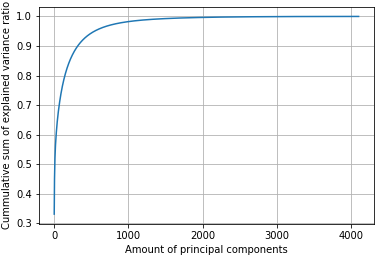
\includegraphics[width = 7 cm]{entities/SHG_pca_var_dist.png}
        \caption{Stacked hourglass}
    \end{subfigure}
    \begin{subfigure}{7 cm}
        \centering
        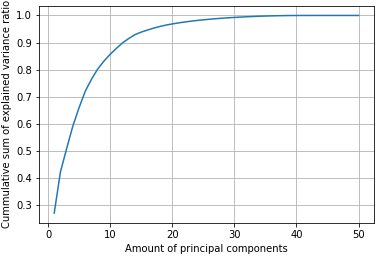
\includegraphics[width = 7 cm]{entities/SHG_AE_pca_var_dist.png}
        \caption{Autoencoder}
    \end{subfigure}
    \caption{Cummulative sum of the explained variance ratio per principal component of the latent space of the Stacked hourglass and autoencoder, respectively}
    \label{fig:sum_cum_distributions}
\end{figure}
\noindent In Section \ref{subsec:shape_analysis} we argued, that the latent space of the developed Stacked hourglass contained a lot of principal components that acted as noise. By using an autoencoder this noise should be removed, since the autoencoder learns the most important features of the input data, as the output of the autoencoder is only an approximation of the input.
\\
\\
In Figure \ref{fig:sum_cum_distributions} we have visualized the cummulative sum of the explained variance ratio per principal component of the latent space of the Stacked hourglass and the autoencoder for the training data. We can clearly see how the autoencoder needs a lot less principal components to represent the data, than the Stacked hourglass. If we assume, that $5\%$ of variance of the data acts as noise, the autoencoder needs $16$ principal components to explain the remaining $95\%$ of the variance of the data, where the Stacked hourglass needs a total of $541$. This means, that by using the autoencoder we have removed a lot of redundancy in the form of noise, essentially denoising the data, which could explain the improvement of the performance.
\\
\\
\\
\\
To sum up, it seems, that we by using the autoencoder in the Stacked hourglass, have improved the structure of the latent space of the model, as well as removed the noise of the latent space, which seems to have improved the performance, as argued in Section \ref{subsec:improv_motivation}.

\subsection{Future Work}\label{subsec:Future_work}
If we were to work further with this project, it would be ideal to explore the effects of stacking multiple modified hourglasses end-to-end. By doing so we would not only hope that the performance of the model to increase further, but we would also hope we could obtain the same accuracy as Newell \textit{et al.} experiences \cite{Newell}, however with fewer stacks. For instance, we could hope that by stacking $2$ modified hourglasses, we would achieve the same results as Newell \textit{et al.}  \cite{Newell} achieves with $4$ hourglasses. In correlation to this, it would also be ideal to examine if any redundancy is added when multiple modified hourglasses are stacked. For instance, if we were to stack $2$ modified hourglasses, maybe only $25$ filters are needed in the second hourglass.
\\
\\
Secondly, one could check for redundancy in the other parts of the model. In Section \ref{sec:XAI} and Section \ref{sec:improving}, we found redundancy in the bottleneck of the model, however, we did not search for any redundancy in the other parts of the model, such as the encoder, decoder and skip-connections, leaving some potential future work. In addition to this, one could retrain a new Stacked hourglass without skip-connections, unilke our procedure in Section \ref{subsec:verifying_skip_cons}, where we simply disabled the skip-connections of an already trained network. This would give less biased results, as well as better insight into the effects of the skip-connects, in comparison to our procedure.
\\
\\
Lastly, it would be interesting to get an understanding of how much of a performance increase one could obtain by using the autoencoder in the hourglass. We described in Section \ref{subsec:why_improvement}, how the latent space of the autoencoder still has some missclassifications, hinting towards some potential increase of performance. If one could correct these missclassifications, how much of an increase in performance would this result in?

\end{document}